\documentclass{article}
\usepackage{graphicx}
\usepackage{enumerate}
\usepackage{cite}


\begin{document}

\title{CMPUT 660 Assignment 1}
\author{Logan Gilmour}

\maketitle

%\begin{abstract}
%The abstract text goes here.
%\end{abstract}

\section{Schema}

I used the MSR Mining Challenge 2013 StackOverflow Posgresql dump\cite{MSRChallenge2013}.

Though there are only four tables in the schema given, both the Votes and Posts tables contain a 'Type Id' field.

By counting the non-null values for each column for each post type, I was able to infer which fields were only present in specific types of posts. Specifically, the 'Question' type has several fields not found in any other type. There are also only three types of posts with comments; the 'Commentable Posts' class is a synthetic construct to indicate that.

Votes also have distinct types (see table), however, they all have the same fields, so I have left them as one class with the type field intact. I have shown the sepparate vote types and their individual counts in the next section.

In order to make the schema more presentable in the UML diagram given here, I replaced all underscores with spaces. All tables also contain Id fields which are not shown.

Field that refer to Ids from different tables are turned into arrows, and inverted to make more sense as a composite structure. For example, the 'post id' field in the 'votes' table became a 'votes' composition on the 'posts' table.

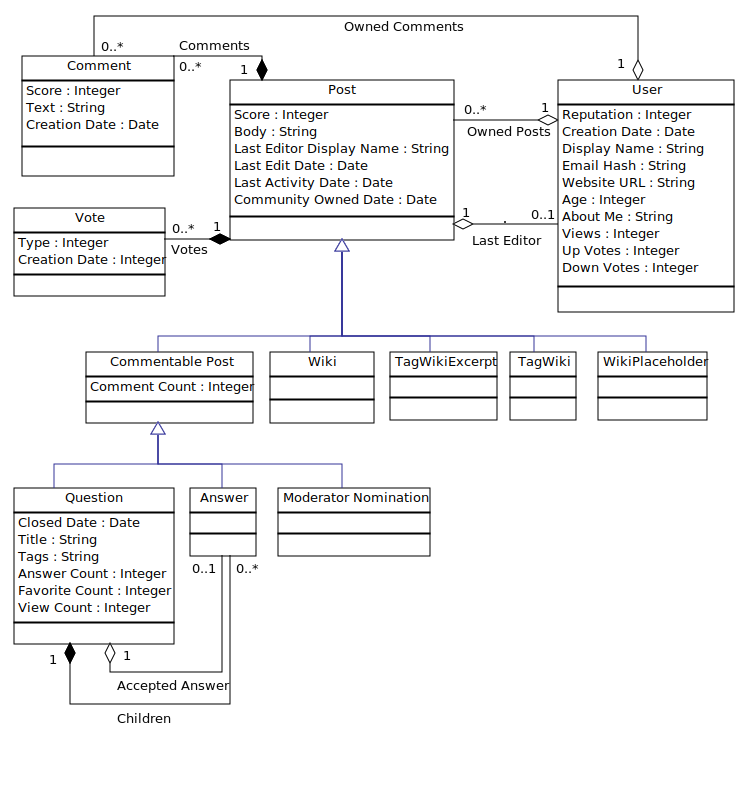
\includegraphics[width=\linewidth]{ClassDiagram}

\newpage

\section{Size Metrics}

\subsection{Counts}

\begin{table}[h]
\begin{minipage}[t]{0.45\linewidth}
\begin{tabular}[t]{| l | r |}
\hline
\multicolumn{2}{|c|}{Posts} \\ \hline
\bf{Type} & \bf{Count} \\ \hline
Question & 3453742 \\ \hline
Answer & 6858133 \\ \hline
Wiki & 167 \\ \hline
TagWikiExcerpt & 13095 \\ \hline
TagWiki & 13095 \\ \hline
ModeratorNomination & 138 \\ \hline
WikiPlaceholder & 1 \\ \hline 
\bf{Total} & 10338371 \\ \hline 
   
\end{tabular}

\vspace{\baselineskip}

\begin{tabular}[t]{| c |}
\hline
Users  \\ \hline
1295620 \\ \hline   
\end{tabular}


\vspace{\baselineskip}


\begin{tabular}[t]{| c |}
\hline
Comments  \\ \hline
13252467 \\ \hline   
\end{tabular}


\end{minipage}
\hspace{0.5cm}
\begin{minipage}[t]{0.45\linewidth}

\begin{tabular}[t]{| l | r |}
\hline
\multicolumn{2}{|c|}{Votes} \\ \hline
\bf{Type} & \bf{Count} \\ \hline
AcceptedByOriginator& 2152420  \\ \hline    
UpMod& 19948316  \\ \hline    
DownMod& 1508097 \\ \hline    
Offensive& 513 \\ \hline    
Favorite& 1877602 \\ \hline    
Close& 475359 \\ \hline    
Reopen& 3327 \\ \hline    
BountyStart& 38358 \\ \hline    
BountyClose& 37959 \\ \hline    
Deletion& 994180 \\ \hline    
Undeletion& 65192 \\ \hline    
Spam& 1946 \\ \hline    
ModeratorReview& 194570 \\ \hline    
ApproveEditSuggestion& 273861 \\ \hline 
\bf{Total} & 27571700 \\ \hline   
\end{tabular}
\end{minipage}
\end{table}

\subsection{Summary Statistics}

I have focused on the Question and Answer types of posts for this section, as they comprise actual question and answer data of StackOverflow.

\begin{tabular}[t]{| l | r |r|r|r|r|} \hline
\multicolumn{6}{|c|}{Questions} \\ \hline
& \bf{Score} & \bf{Comment Count} & \bf{Favorite Count} & \bf{Answer Count} & \bf{View Count} \\ \hline
min  &           -132 &       0 &        0 &       0 &        1 \\ \hline
max  &           2499 &     109 &     5894 &     519 &  1051784 \\ \hline
median &            1 &       0 &        0 &       2 &      205 \\ \hline
mean  &             1.4952 &       1.3276 &        0.5178 &       1.986 &      730.1 \\ \hline
var   &            45.1488 &       4.5475 &       41.1802 &       3.550 & 10825646.4 \\ \hline
std.dev  &          6.7193 &       2.1325 &        6.4172 &       1.884 &     3290.2 \\ \hline
skewness & 81.4  &          2.9  &        401.1  &         20.6  &         43.6  \\ \hline
kurtosis & 15366   &          21  &       279068   &        3299    &       5516 \\ \hline
\end{tabular}

\vspace{\baselineskip}

\begin{tabular}[t]{| l | r |r|} \hline
\multicolumn{3}{|c|}{Answers} \\ \hline
& \bf{Score} & \bf{Comment Count} \\ \hline 
min & -59    &   0 \\ \hline
max      &        4432  &   133 \\ \hline
median      &        1  &     0 \\ \hline
mean          &      1.8672   &    1.26376 \\ \hline
var        &        53.1593   &    4.25170 \\ \hline
std.dev      &       7.2910   &    2.06196 \\ \hline
skewness & 117.8    &       3.5  \\ \hline
kurtosis & 37770     &       34  \\ \hline
\end{tabular}

\vspace{\baselineskip}

\begin{tabular}[t]{| l | r |r|r|} \hline
\multicolumn{4}{|c|}{Users} \\ \hline
& \bf{Views} & \bf{Up Votes} & \bf{Down Votes} \\ \hline 
min      &          0  &      0 &      0  \\ \hline 
max      &     195496  &  17587 &  91092  \\ \hline 
median       &      0 &      0  &    0  \\ \hline  
mean         &      6.92   &    15.40 &      1.164  \\ \hline 
var       &     44714.20  &  19512.37  &  7141.739  \\ \hline 
std.dev     &     211.46  &    139.69 &     84.509  \\ \hline 
skewness & 643   &      31   &     971  \\ \hline 
kurtosis & 569104   &    1741 &   1042095  \\ \hline 
\end{tabular}

\section{Tracebility}

To find bug and issue IDs, I adapted the bug ID regex given by Fischer et al. \cite{fischer}

Hyperlinks
Bug/Issue ids
Files
Projects?

\begin{tabular}[t]{| l | r | r | r |}
\hline
\multicolumn{4}{|c|}{Post Body} \\ \hline
\bf{Type} & \multicolumn{3}{|c|}{\bf{Count}} \\ \hline
 & Email Addresses & Issue IDs & Hyperlinks \\ \hline
Question & 49748 & 608 & 12130779 \\ \hline
Answer & 30847 & 2321 & 12252559 \\ \hline
Wiki &  0 & 0 & 92\\ \hline
TagWikiExcerpt & 0 & 0 & 728\\ \hline
TagWiki & 19 & 1 & 21194\\ \hline
ModeratorNomination & 1 & 0 & 272 \\ \hline
WikiPlaceholder & 0 & 0 & 9\\ \hline
Total& 80615 & 2930 & 24405633 \\ \hline      
\end{tabular}

\vspace{\baselineskip}

\begin{tabular}[t]{| l | r | r | r |}
\hline
\multicolumn{4}{|c|}{Comment Text} \\ \hline
\bf{Parent Type} & \multicolumn{3}{|c|}{\bf{Count}} \\ \hline
 & Email Addresses & Issue IDs & Hyperlinks \\ \hline
Question & 2675 & 285 & 1241586 \\ \hline
Answer &  5680 & 539 & 2128905 \\ \hline
ModeratorNomination & 0 & 0 & 282 \\ \hline
Total& 8355 & 824 & 3370774 \\ \hline      
\end{tabular}

\bibliography{resources}{}
\bibliographystyle{plain}

\end{document}
